\documentclass{article}
\usepackage[utf8]{inputenc}
\usepackage{amsmath}
\usepackage{amsfonts}
\usepackage{amssymb}
\usepackage{blindtext}
\usepackage{biblatex}
\usepackage{subfig}
\usepackage{graphicx}
\title{Project 1 - Regression analysis and resampling methods}
\author{Espen Ulset Nordsveen
\and Ghadi Al Hajj}

\DeclareRobustCommand{\bbone}{\text{\usefont{U}{bbold}{m}{n}1}}

\DeclareMathOperator{\EX}{\mathbb{E}}

\begin{document}
\maketitle
\section{Introduction}
Linear regression is an important tool within the field of statistics and data analysis. This statistical method aims to determine the strength and character of the relationship between one dependent variable, also called the outcome, and one or more independent variables, also called the features. This is achieved by mapping this relationship through a mathematical formula that best approximates the data points within a given data set.

This tool is used in several fields of science spanning medicine, physics, finance, astronomy...

In this project, our goal was to analyse and compare the performance of various linear regression methods, namely the Ordinary Least Squares (OLS), Ridge regression and the Lasso regression. These methods were combined with resampling techniques like the bootstrap and cross validation techniques to get better estimates of the error, specifically on the test data. In addition, bootstrap was used to perform a bias-variance tradeoff analysis for all methods.

\subsection{Linear Regression}
As mentioned, linear regression attemps to find a relationship between two or more variables by fitting a linear equation to observed data. We denote the dependent variable, or outcome, as $\textbf{y}$. If we have a set of independent variables, or features, $\textbf{X}^{T} = (X_{1}, X_{2}, \dots, X_{p})$, and assuming a linear relationship between these, the $y$ can be predicted as
\begin{equation} \label{ytilde}
\tilde{y} = \tilde{\beta_{0}} + \sum_{j=1}^{p} X_{j} \tilde{\beta_{j}}
\end{equation}
By including the constant variable 1 in $X$, and include $\tilde{\beta_{0}}$ in the vector of coefficients $\tilde{\beta}$,  (\ref{ytilde}) can be written in vector form as
\begin{equation}\label{matrixform}
\textbf{y} = \textbf{X} \beta + \epsilon
\end{equation}
where $\epsilon$ denotes the residual error of the linear model $\textbf{X}\beta$ from the true response, and the $\beta$ is the parameter vector containing the linear regression coefficients $\beta_{i}$. $y$ and $\epsilon$ are defined as the following vectors
\begin{equation}
\textbf{y} = [y_{0}, y_{1}, y_{2}, \dots, y_{n-1}]^{T}
\end{equation}

\begin{equation}
\beta = [\beta_{0}, \beta_{1}, \beta_{2}, \dots, \beta_{n-1}]^{T}
\end{equation}

\begin{equation}
\epsilon = [\epsilon_{0}, \epsilon_{1}, \epsilon_{2}, \dots, \epsilon_{n-1}]^{T}
\end{equation}
and $\beta$ are in fact the unknown parameters in the linear regression problems that needs to be calculated. The $X$ matrix in (\ref{matrixform}) can be expressed as
\begin{equation} \label{designM}
\textbf{X} = 
\begin{bmatrix}
1 & x_{0}^{1} & x_{0}^{2} & \dots & x_{0}^{n-1} \\
1 & x_{1}^{1} & x_{1}^{2} & \dots & x_{1}^{n-1} \\
1 & x_{2}^{1} & x_{2}^{2} & \dots & x_{2}^{n-1} \\
\vdots & \vdots & \vdots & \dots & \vdots \\
1 & x_{n-1}^{1} & x_{n-1}^{2} & \dots & x_{n-1}^{n-1} \\ 
\end{bmatrix}
\end{equation}
With the design matrix defined as (\ref{designM}), we can use this together with the unknown $\beta$ to approximate $y$ as
\begin{equation}
\textbf{\~{y}} = \textbf{X}\beta
\end{equation}
We see that
\begin{align}
\tilde{y} &= \textbf{X}\beta \\
&= y - \epsilon
\end{align}
We therefore need to find $\beta$ values such that the error $\epsilon$ is minimized, which indeed is the true objective of linear regression.

\subsection{Ordinary Least Squares}\label{OLSsection}
The ordinary least square (OLS) method is defined by the following cost function [Hjort-Jensen]
\begin{equation}\label{costfunctionOLS}
C(\beta) = \frac{1}{n} \sum_{i=0}^{n-1} (y_{i} - \tilde{y}_{i})^{2} = \frac{1}{n} \{ (\textbf{y} - \tilde{y})^{T} (\textbf{y} - \tilde{y} \}
\end{equation}
In matrix-vector notation, this becomes
\begin{equation}\label{costfunctionOLS2}
C(\beta)= \dfrac{1}{n} \{( \textbf{y}-\textbf{X}\beta^{T}\textbf{y}-\textbf{X}\beta)\}
\end{equation}
By minimizing this cost function, this is in fact a estimation of the parameters $\beta$ by minimizing the sum of the squared residuals. The minimization problem of the cost function (\ref{costfunctionOLS2}) is solved by derivation of the function. The derivatives of (\ref{costfunctionOLS2}) gives the parameterization of $\beta$ for the OLS method as
\begin{equation}\label{betaOLS}
\beta = (\textbf{X}^{T}\textbf{X})^{-1}\textbf{X}^{T}\textbf{y}
\end{equation}
We see from (\ref{betaOLS}) that finding an approximation for $\beta$ involves a matrix inversion. In cases where $\textbf{X}^{T}\textbf{X}$ is singular, it is non-invertible, and the parameterization of $\beta$ in (\ref{betaOLS}) can not be calculated. In these cases, the \textit{Singular Value Decomposition} (SVD) can be used. The SVD decompose any matrix \textbf{X} with dimension $P \times n$ into terms of a diagonal matrix and two orthogonal matrices, leading to the expression [Hastie et al.]
\begin{equation}
\textbf{X} = \textbf{U} \textbf{D} \textbf{V}^{T}
\end{equation}
Here $\textbf{U}^{N \times p}$ and $\textbf{V}^{p \times p}$ are orthogonal matrices, with the columns of \textbf{U} spanning the column space of \textbf{X}, and the columns of \textbf{X} spanning the row space. $\textbf{D}^{p \times p}$ is a diagonal matrix. In this study, SVD was used wherever the resulting matrices were non-invertible using the \verb+np.pinv()+ function from the \verb+numpy+ library.

\subsection{Bias-Variance Tradeoff}
For continuous predictions, we can assume that the true data is generated from a noisy model as [Hjort-Jensen]
\begin{equation}
y = f(x) + \epsilon
\end{equation}
where $\epsilon$ is normally distributed with mean zero and standard deviation $\sigma^{2}$. We saw from the OLS method in section \ref{OLSsection} that $f$ can be approximated in terms of $\beta$ and the design matrix $\textbf{X}$ as $\tilde{\textbf{y}} = \textbf{X} \beta$. We then found the parameters $\beta$ by minimizing the cost function
\begin{equation}\label{biastradeoff}
C(\textbf{X},\beta) = \frac{1}{n} \sum_{i=0}^{n-1} (y_{i} - \tilde{y}_{i})^{2} = \EX [(\textbf{y} - \widetilde{\textbf{y}})^{2}]
\end{equation}
This can be rewritten as
\begin{align*}\label{biastradeoff}
C(\textbf{X},\beta) &= \EX [(\textbf{y} - \widetilde{\textbf{y}})^{2}]\\
&= \dfrac{1}{n} \{( \textbf{y}-\textbf{X}\beta^{T}\textbf{y}-\textbf{X}\beta)\} \\
&= \EX [(f + \epsilon - \tilde{\textbf{y}})^{2}] \\
&= \EX [(f + \epsilon - \tilde{\textbf{y}} + \EX[\tilde{\textbf{y}}] - \EX[\tilde{\textbf{y}}])^{2}]\\
&= \EX [(\textbf{y} - \EX [\tilde{\textbf{y}}])^{2} + Var[\tilde{\textbf{y}}] + Var[\epsilon^{2}] \\
&= \frac{1}{n} \sum (f_{i} - \EX[\tilde{\textbf{y}}])^{2} + \frac{1}{n} \sum (\tilde{\textbf{y}} - \EX[\tilde{\textbf{y}}])^{2} + \epsilon^{2} \\
&= \frac{1}{n} \sum (f_{i} - \EX[\tilde{\textbf{y}}])^{2} + \frac{1}{n} \sum (\tilde{\textbf{y}} - \EX[\tilde{\textbf{y}}])^{2} + \sigma^{2}
\end{align*}
We see that the first part is the difference between the expected value of the model prediction and the true value of $y$, and is called the \textit{bias}. The value is used for evaluation of the predicted model. A bias of zero is called unbiased, and will thus not contain any systematic or random errors, which is fairly unlikely. The second part is the squared deviation of $y$ from its mean, which is called the {variance}. It basically describes the spread of the prediction.

\subsection{Ridge Regression}
Ridge regression is a method for shrinking the regression coefficients by imposing a penalty on their size. The Ridge coefficients minimize a penalized residual sum of squares. This circumvent the problem with colinearity we saw for the OLS method, where $\textbf{X}^{T}\textbf{X}$ might be singular. This is especially true for higher dimensions of the design matrix. By adding a penalty factor $\lambda$ to the diagonal of $\textbf{X}^{T}\textbf{X}$, the term is always invertible. The cost function for ridge regression can be expressed as
\begin{equation}
C(\textbf{X},\beta) = \dfrac{1}{n} \{( \textbf{y}-\textbf{X}\beta^{T}\textbf{y}-\textbf{X}\beta)\} + \lambda \beta^{T} \beta 
\end{equation}
and the parameterization for the ridge method thus become
\begin{equation}
\beta = (\textbf{X}^{T}\textbf{X} + \lambda\textbf{I})^{-1}\textbf{X}^{T}\textbf{y}
\end{equation}
We see that a diagonal matrix including the penalty factor $\lambda$ is added to $\textbf{X}^{T}\textbf{X}$. 
\subsection{Lasso Regression}
As for Ridge regression, Lasso is also a shrinkage method. Lasso stands for "Least Absolute Shrinkage and Selection Operator", and like Ridge, it fits the linear regression model by minimizing the sum of the squares augmented with a penalty factor. However, in Lasso regression, the penalty function becomes non-linear. In contrast to the Ridge regression, it is in fact the absolute values of the regression parameters multiplied by the penalty factor $\lambda$ [Wieringen]. There is no analytical expression for finding $\beta$, but is in fact done iteratively. 
\subsection{The Bootstrap}
The boostrap resampling method is a simple Monte Carlo technique to approximate the sampling distribution (KILDE). The method randomly draw $B$ datasets with replacement from the training data, where each sample is the same size as the original training set. The model is then refit to the $B$ bootstrap datasets \cite{Hastie et al.}. In the context of this project, we use this method to calculate MSE, bias and variance of the model.
\subsection{\textit{k}-fold Cross Validation}
The $k$-fold Cross Validation technique is a resampling procedure used to evaluate the performance of statistical models on a limited data sample. The method generally results in a less biased or less optimistic estimate of the model compared to other methods, such as the train/test split. The \textit{k} refers to the equally number of groups the given sample shall be split into. One of these groups are set aside as the validation group. The rest of the groups, i.e. $K-1$, are used to fit the model, and calculate the prediction error of the fitted model when predicting the $k$th part of the data. A normal value for $k$ is $K=5$, as this gives a lower variance. It might, however, give problems with the bias if the training sets becomes too small.

The general procedure for the $k$-fold Cross Validation is as follows (KILDE)
\begin{enumerate}
\item Shuffle the dataset
\item Split the dataset into $k$ groups
\item For each unique group
\begin{enumerate}
\item Take the group as a hold out or test data set
\item Take the remaining groups as a training data set
\item Fit a model on the training set and evaluate it on the test set
\item Retain the evaluation score and discard the model
\end{enumerate}
	
\item Summarize the skill of the model using the sample of model evaluation scores
\end{enumerate}

\subsection{Model analysis}
To evaluate how well the predicted model fits the real data, we need to define some measures to be evaluated
\subsubsection{Mean Squared Error}
The mean squared error (MSE) of an estimator is the averaged squared difference between the estimated values and the actual value. That is, the difference between the predicted data points $\tilde{\textbf{y}}$ and their actual value $\textbf{y}$, and is defined by
\begin{equation}\label{MSE}
MSE = \frac{1}{n} \sum_{i=0}^{n}(y_{i} - \tilde{y}_{i})^{2}
\end{equation}
MSE values close to zero thus indicates a pretty good estimate for the model.
\subsubsection{$R2$-score}
The R2 value, or the \textit{coefficient of determination}, measures how well future values are likely to be predicted by the model. It is a relationship between the variance of the predicted model and the total variance of the input data, and is defined by
\begin{equation}\label{R2score}
R^{2} = 1-\frac{\sum_{i=0}^{n}(y_{i} - \tilde{y}_{i})^{2}}{\sum_{i=0}^{n}(y_{i} - \bar{\textbf{y}}_{i})^{2}}
\end{equation}
where $\overline{y}$ is defined as
\begin{equation}
\overline{y} = \dfrac{1}{n} \sum_{i=0}^{n-1} y_{i}
\end{equation}
The $R^{2}$ score might be positive or negative. A score of 1 is the best possible score, and indicates that the predictions perfectly fits the data. A constant model that always predicts the expected value of $\tilde{y}$ without caring for the input data, get a $R^{2}$ score of 0.
\subsection{Confidence interval}
The confidence interval gives an estimate of how well $\beta$ is predicted. The $95\%$ confidence interval for $\beta_{j}$ can be defined as [Hastie et al.]
\begin{equation}
c_{\beta_{j}} = \beta_{j} \pm 1.645 \sigma
\end{equation}
It gives an confidence level that the true parameter is in the proposed range. 
\section{Data}
\subsection{Franke's function}
The Franke's function will be used as a basis for our discussion of the various regression and resampling methods in this context. This is a function  widely used as a test function in interpolation problems, and is defined by

\begin{align*}
f(x,y) &= \frac{3}{4}exp\left(-\frac{(9x-2)^2}{4} - \frac{(9y-2)^2}{4}\right)+\frac{3}{4}exp\left(-\frac{(9x+1)^2}{49} - \frac{(9y+1)}{10}\right)\\
&+ \frac{1}{2}exp\left(-\frac{(9x-7)^2}{4} - \frac{(9y-3)^2}{4}\right)-\frac{1}{5}exp\left(-(9x-4)^2 - (9y-7)^2\right)
\end{align*}
\section{Method}
The Franke function is a multivariable function, depending on both $x$ and $y$, and hence is a 2-variable polynomial. The design matrix in (\ref{designM}) thus needs to be adjusted for this multivariable case. The design matrix thus becomes  
$$\textbf{X} = \begin{bmatrix}
1 & x_{0} & y_{0} & x_{0}y_{0} & \dots & x_{0}^{N} & y_{0}^{N}     \\
1 & x_{0} & y_{1} & x_{0}y_{1} & \dots & x_{0}^{N} & y_{1}^{N}  \\
\vdots & \vdots & \vdots & \vdots & \dots & \vdots & \vdots \\
1 & x_{1} & y_{0} & x_{1}y_{0} & \dots & x_{1}^{N} & y_{0}^{N} \\
\vdots & \vdots & \vdots & \vdots & \dots & \vdots & \vdots \\
1 & x_{n-1} & y_{m-1} & x_{n-1}y_{m-1} & \dots & x_{n-1}^{N} & y_{m-1}^{N} \\
\end{bmatrix}$$
where $N$ is the polynomial degree.

\section{Results}
\subsection{Ordinary least squares on the Franke Function}
In this part, we performed the plain OLS regression on the data that is generated using the Franke function. Before that, we split the data into training set, on which the model is trained, and a testing sets, on which the model’s performance is evaluated for the goodness of the fit. The ratio of training to testing sets 70/30. The same train/test split was done in all the coming parts to ensure a fair and reproducible comparison between the different methods. This was achieved by using the same random seed in all the cells.

\begin{figure}[h]
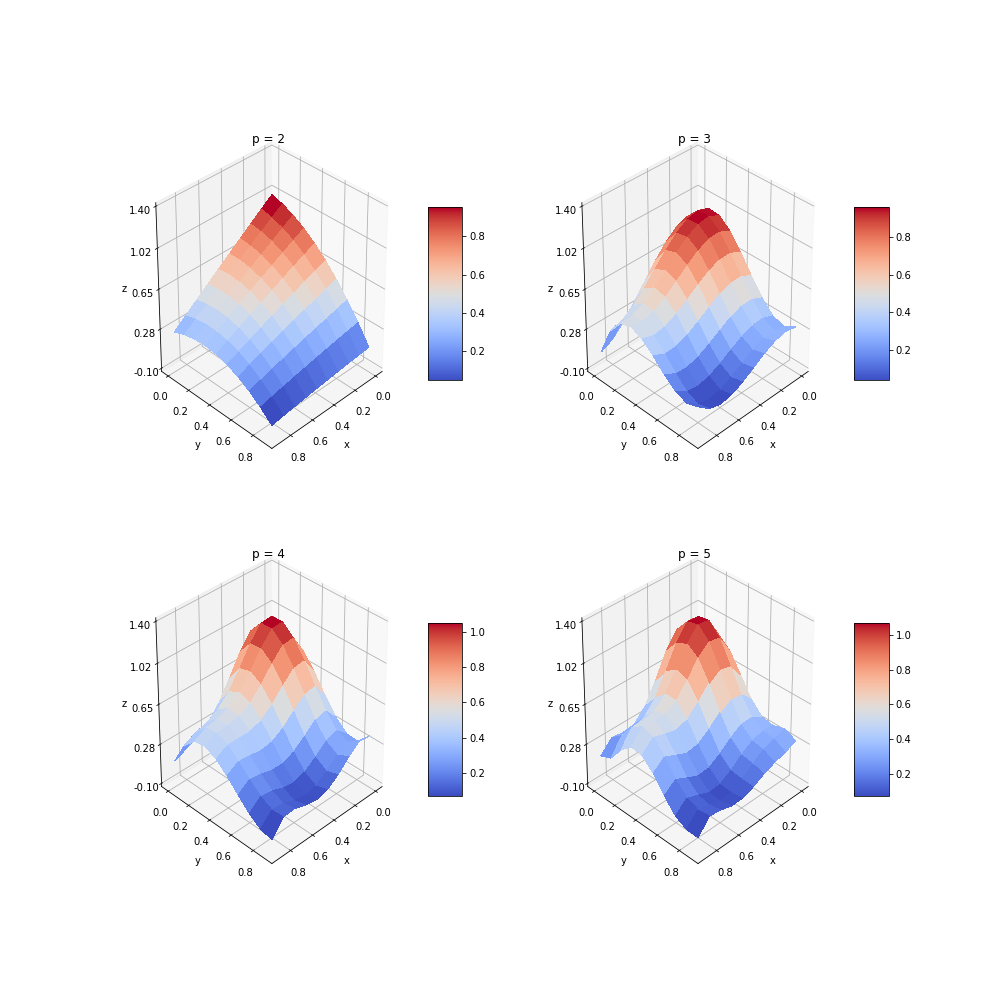
\includegraphics[scale=0.35]{frankePlots.png}
\caption{OLS on the Franke function, with increasing polynomial degree}
\end{figure}

For performing the OLS, a polynomial of degree five was used to generate the features of the model, and then these features were scaled according to the training data statistics, in order to force the data into a distribution with zero mean and unit variance. This is useful because it ensures that each feature gets an equal chance of being represented in the polynomial, thus preventing features with large values to dominantly control the shape of the polynomial.

The metrics were then applied to both sets and the R2 coefficient and the Mean Square Error of each set were calculated. In addition, we generated a plot of the confidence intervals of the tunable parameters, shown in figure \ref{fig:confintOLS}. The Mean Square error was calculated by (\ref{MSE}) and the R2 coefficient was calculated by (\ref{R2score}).
\begin{figure}
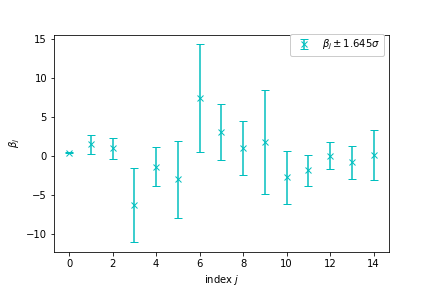
\includegraphics[scale=0.5]{confidenceintervall.png}
\centering
\caption{Confidence intervall of the tunable paramteres}
\label{fig:confintOLS}
\end{figure}
In our demonstration, we noticed that if the design matrix is created from data points within the range of [0,1], then the resulting  matrix would be close to singularity, and the program would thus raise an error whenever the inverse is calculated, particularly when calculating  or its variance. This, in turn, caused the problem of getting negative values for the variance of some values. Using pinv, however, instead of inv, solved both problems when calculating the inverses.

It is also worth mentioning that when the range of values that the raw features can take is increased to, say, [0,5], instead of [0,1], the problem of singular matrices immediately disappears even when using inv and the determinant of the matrix  becomes greater than zero.



\subsection{Bias-variance trade-off and resampling techniques}
When evaluating the model’s performance on the test data that the model has not seen before, we want to measure the difference/error between the model’s predictions and the true values. This error can be split into three terms.

The bias term is a quantity that describes how much the data is shifted from the mean value of the model. A high bias indicates that the model is not able to represent the patterns in the underlying data.

Variance, on the other hand, represents the variance of the predicted data from its corresponding mean, and it describes the sensitivity of the model to the noise in the data. Thus, high variance indicates that the model has not only learned the underlying model, but went further to even capture the noise in the data.

A model that is simple and does not capture the underlying trends in the data is called an underfitting model, and has high bias and low variance. On the other hand, a model that is too complex will likely result in overfitting, in which case it would have low bias and high variance.

Last is the irreducible error term. This represents the error that is not related to the complexity of the model and that cannot be reduced no matter how good and tuned the model is, with a given set of predictors. This error term is given by the variance of the noise in the data, and can be reduced by recognizing more independent predictors that are also related to the dependent variable.

Figure \ref{fig:plot} (add figure for bias variance tradeoff) shows the trends in the bias and the variance as a function of the model’s complexity. 

As expected, at low degrees of complexity, the model suffers from under-fitting as a low order polynomial cannot reasonably represent a complex function with exponential and quadratic terms. This is shown by the high bias for polynomials of low order.

As the complexity increases, the bias starts decreasing indicating that the model is no longer deficient of approximating the overall shape and trends in the data. At a certain polynomial degree (5), the model reaches a balance between bias and variance, where the overall error is the lowest. Such a model is a model that has learned the trends in the data but has not yet entered the stage of memorizing the training data and adapting itself to the noise/idiosyncrasies in the training data.

When the polynomial degree exceeds 5, the variance starts to increase in value indicating that the model has now entered into the realm of over-fitting. This variance will keep increasing as the complexity increases until the model has learned all the noise in the training data. This additional learning negatively impacts the model’s performance on new data and inhibits its ability to generalize to the domain of interest, which is the ultimate goal of any machine learning algorithm.

\begin{figure}[h]\centering
\subfloat[legend]{\label{a}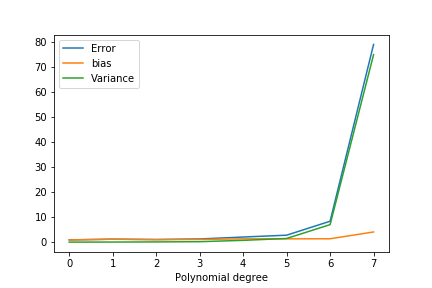
\includegraphics[width=.45\linewidth]{partBplot10.png}}\hfill
\subfloat[legend]{\label{b}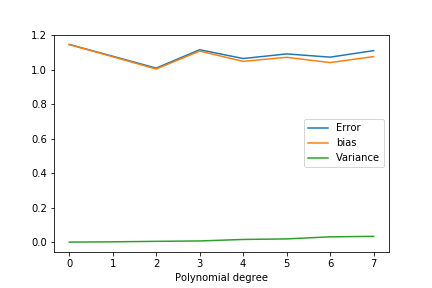
\includegraphics[width=.45\linewidth]{partBplot40.png}} \par
\subfloat[legend]{\label{c}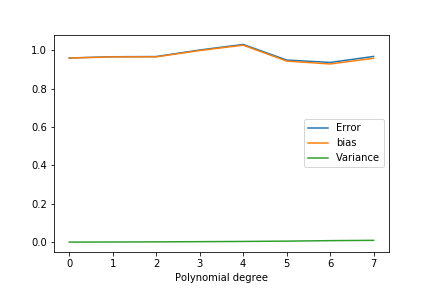
\includegraphics[width=.45\linewidth]{partBplot70.png}}\hfill
\subfloat[legend]{\label{c}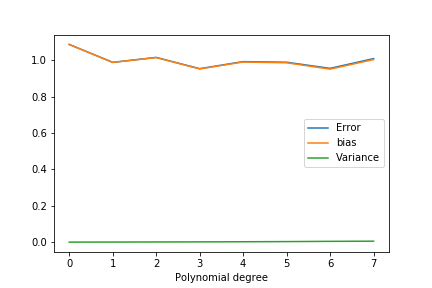
\includegraphics[width=.45\linewidth]{partBplot100.png}}\par
\caption{Plots of the relationships between error, bias and variance with bumber of bootstraps = 200, using the bias-variance tradeoff}
\label{fig}
\end{figure}





\subsection{Cross-validation as resampling techniques}
In this part, we performed a k-fold cross validation analysis to estimate the value of the Mean Square Error of our model of a seventh degree polynomial. We estimated this quantity using 5 and 10 folds.

The cross validation analysis gives estimates of 0.0033 and 0.0021, for 5- and 10-folds, respectively, which are both relatively lower than the estimate of this quantity from bootstrap at the same model complexity, 0.1019. This illustrates the fact that cross validation gives an over optimistic estimate for this error.

It is also important to note that the bootstrap approach is closer to the real scenario because after each bootstrapping iteration, the model is tested on the same test set, whereas in cross validation, each time the test set is changed.

\clearpage
\subsection{Ridge regression on the Franke function with resampling}
In this part, we used the same data from a Franke function to study the effect of L2 regularization, i.e. Ridge regression, on the output model and its performance.

For the hyper-parameter $\lambda$, we used four different values on a log-scale from -4 to 1 to create four different models. Specifically, these corresponds to the values 1.0 e-04, 4.6 e-03, 2.2 e-01, and 1.0.

From figure \ref{RidgeConfInt}, it can be seen that as the value of $\lambda$ increases the parameters beta and their confidence intervals become more centered around zero. This is because a higher value of  places a higher penalty on high values of , thereby preventing it from taking large values, which can lead to over-fitting.
\begin{figure}[ht]\centering
\subfloat[$\lambda=0.0001$]{\label{a}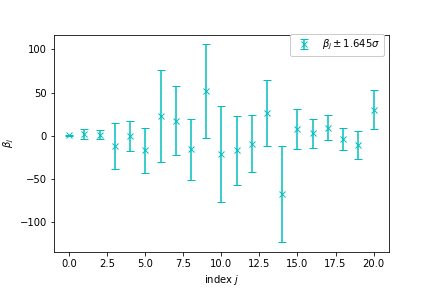
\includegraphics[width=.45\linewidth]{CIbetaridgelambda0.0001.png}}\hfill
\subfloat[$\lambda=0.0046$]{\label{b}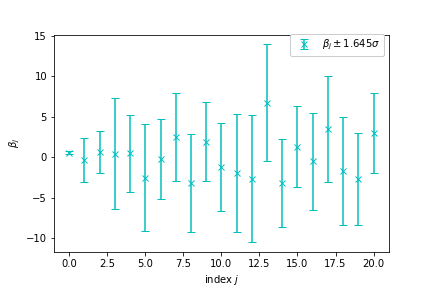
\includegraphics[width=.45\linewidth]{CIbetaridgelambda0.004641588833612782.png}} \par
\subfloat[$\lambda=0.2154$]{\label{c}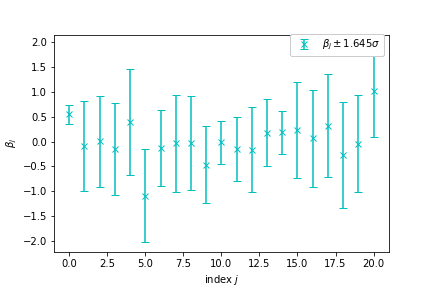
\includegraphics[width=.45\linewidth]{CIbetaridgelambda0.21544346900318845.png}}
\subfloat[$\lambda=10.0$]{\label{c}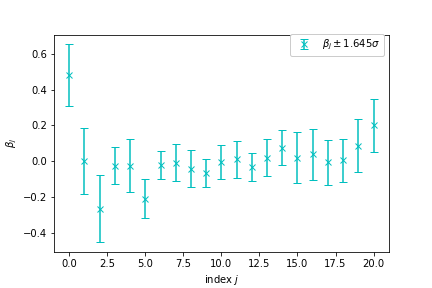
\includegraphics[width=.45\linewidth]{CIbetaridgelambda10.0.png}}
\caption{Plots of the confidence intervall for the ridge regression on the Franke function}
\label{RidgeConfInt}
\end{figure}
In the same analysis, comparing the values of the Mean Squared Error across the used values of  shows that the error on the test set decreases with increasing values of $\lambda$ whereas the error of the training set increases. This is because, as discussed before, L2 regularization fights over-fitting. Therefore, for higher values of , less emphasis is put on reproducing the training data set with its idiosyncrasies and more importance is placed on learning the general patterns in the training data. This, in turn, improves the model’s ability to generalize to data points that it has not seen before during training.

Next, we applied the bootstrapping method to ridge regression to compare it with the results from OLS regression, and study its behavior in the bias-variance trade-off. See figure \ref{Ridgebootstrap}. The same behavior of decreasing bias and increasing variance is observed, though, the bias’s behavior is more evident at low values of noise variance. However, it it also important to note that as the value of $\lambda$ increases it takes the variance additional degrees to emerge and manifest itself. This is, again, expected because regularization fights over-fitting, which a model exhibits when the variance is high.
\begin{figure}[h]\centering
\subfloat[$\lambda=0.0001$]{\label{a}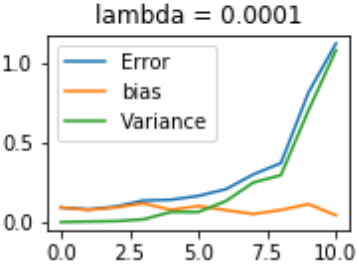
\includegraphics[width=.45\linewidth]{boostrapridge0.png}}\hfill
\subfloat[$\lambda=0.0046$]{\label{b}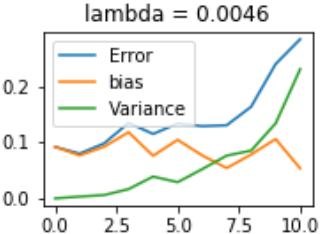
\includegraphics[width=.45\linewidth]{boostrapridge1.png}} \par
\subfloat[$\lambda=0.2154$]{\label{c}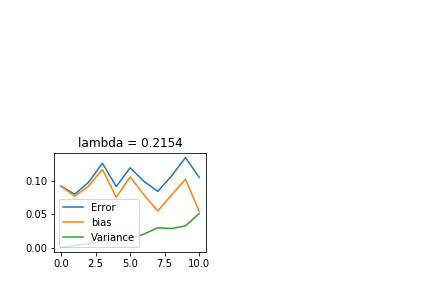
\includegraphics[width=.45\linewidth]{boostrapridge2.png}}\hfill
\subfloat[$\lambda=10.0$]{\label{c}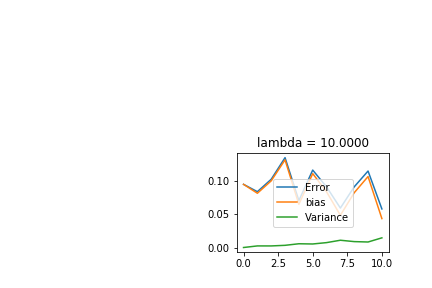
\includegraphics[width=.45\linewidth]{boostrapridge3.png}}\par
\caption{Plots of the relationships between error, bias and variance using Ridge bootstrapping}
\label{Ridgebootstrap}
\end{figure}
Moving into cross-validation, the ridge regression model gives a lower estimate of the MSE than OLS at all values of $\lambda$ and both number of folds, except at $\lambda = 10^{-1}$ with five folds. Moreover, similar to the case with OLS, again, cross-validation gives a lower estimate of the error compared to bootstrap.

\clearpage
\subsection{Lasso regression}
Complementing our study of OLS and Ridge regression, here, we present a similar study on the Franke function data to study the effect of L1 regularization, i.e. Lasso regression, on the resulting model and its performance, see figure \ref{LassoConfInt}. Here, the values of $\lambda$ are the same as those used in Ridge regression.
\begin{figure}[h]\centering
\subfloat[$\lambda=0.0001$]{\label{a}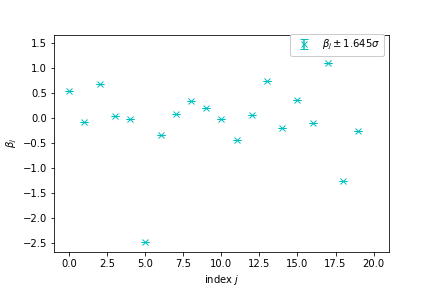
\includegraphics[width=.45\linewidth]{Plots/CIbetalassolambda0.png}}\hfill
\subfloat[$\lambda=0.0046$]{\label{b}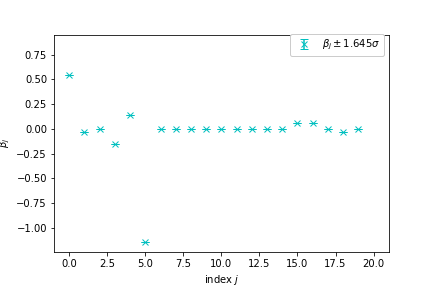
\includegraphics[width=.45\linewidth]{Plots/CIbetalassolambda1.png}} \par
\subfloat[$\lambda=0.2154$]{\label{c}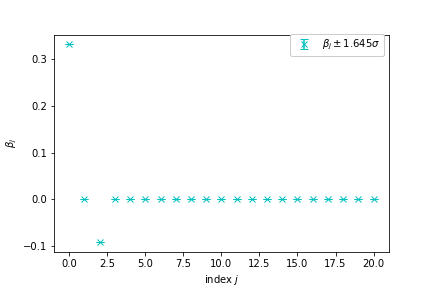
\includegraphics[width=.45\linewidth]{Plots/CIbetalassolambda2.png}}\hfill
\subfloat[$\lambda=10.0$]{\label{c}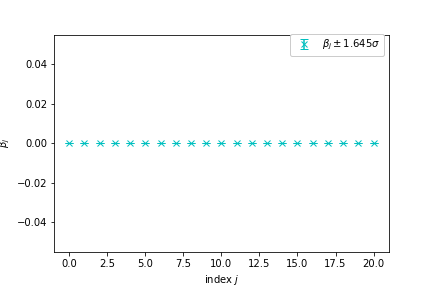
\includegraphics[width=.45\linewidth]{Plots/CIbetalassolambda3.png}} \par
\caption{Plots of the confidence intervall for the lasso regression on the Franke function}
\label{LassoConfInt}
\end{figure}
Similar to Ridge regression, as the value of $\lambda$ increases the parameters beta become more centered around zero, for the same reason of being penalized for having large values. However, the true difference between Lasso and Ridge is that instead of just centering the values of beta around zero, thereby, preventing them from attaining large values, Lasso takes a step further and actually set some parameters to exactly zero. This behavior is more evident at high values of $\lambda$. In this way, Lasso can be seen as a shrinkage and feature selection method.
Here, it is important to note that the confidence intervals were not calculated as there is no analytical equation for this quantity. Instead, only the values of the obtained $\beta$'s are displayed.
\begin{figure}[h]
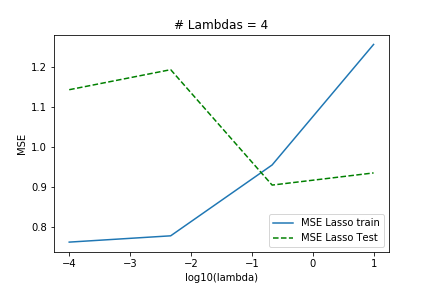
\includegraphics[scale=0.5]{Plots/lassoRegressionModelplot.png}
\centering
\caption{MSE for train and test set for Lasso}
\label{fig:lassoTrainTest}
\end{figure}
Comparing the models built with different values of $\lambda$, we find that Mean Squared Error on the test set decreases with increasing values of $\lambda$, whereas the error of the training set increases. The same reasoning follows here of how L1 regularization fights over-fitting by, thereby finding a balance between reproducing the training data and generalizing to data that it has not been trained on.

For the bias-variance trade-off, we observed a similar behavior of decreasing bias and increasing variance to that observed in Ridge. Again, it takes the variance higher complexity values to become evident.

Finally, in figure \ref{Lassobootstrap} the cross-validation analysis shows that the Lasso regression model, again, gives a lower estimate of the MSE than OLS at all values of $\lambda$ and both number of folds. Moreover, similar to the case with OLS and Ridge, again, cross-validation gives a lower estimate of the error compared to bootstrap.
\begin{figure}[h]\centering
\subfloat[$\lambda=0.0001$]{\label{a}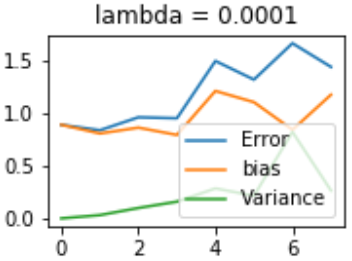
\includegraphics[width=.45\linewidth]{boostraplasso0_cut.png}}\hfill
\subfloat[$\lambda=0.0046$]{\label{b}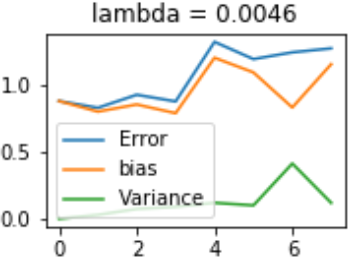
\includegraphics[width=.45\linewidth]{boostraplasso1_cut.png}} \par
\subfloat[$\lambda=0.2154$]{\label{c}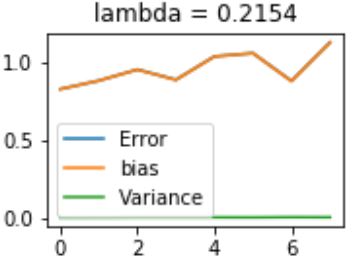
\includegraphics[width=.45\linewidth]{boostraplasso2_cut.png}}\hfill
\subfloat[$\lambda=10.0$]{\label{c}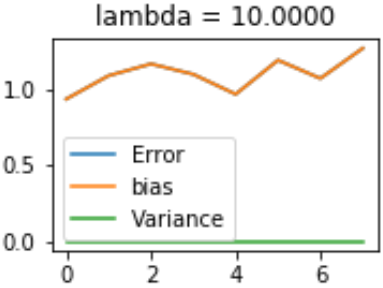
\includegraphics[width=.45\linewidth]{boostraplasso3_cut.png}}\par
\caption{Plots of the relationships between error, bias and variance using Lasso bootstrapping}
\label{Lassobootstrap}
\end{figure}

\clearpage
\subsection{Introducing real terrain data}
Looking beyond the Franke functions from now, and looking into real data, the previous methods will now be tested on terrain data. We use digital terrain data from Norway, see figure \ref{terraindata} for a visual presentation. 
\begin{figure}[h]
\begin{minipage}{0.48\textwidth}
\centering
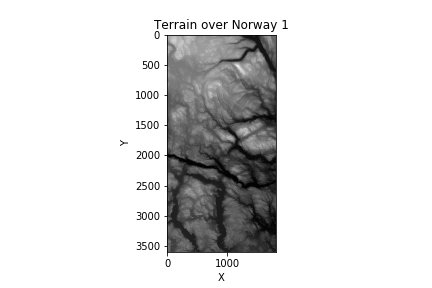
\includegraphics[width=1.5\linewidth]{terrain2dplot.png}
\end{minipage}
\begin{minipage}{\textwidth}

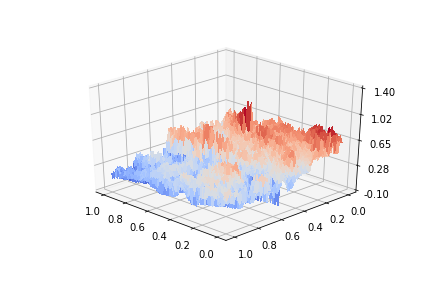
\includegraphics[width=0.7\linewidth]{rawdataplot.png}
\end{minipage}
\caption{2D and 3D plot of the terrain data used as basis for our analysis}
\label{terraindata}
\end{figure}

\clearpage
\subsection{Regression techniques on terrain data}
In this part, we applied all of the three discussed methods on the terrain data. In order to get a general sense of each method's approach in reproducing the terrain data, we used all of the cropped image to train a model of each type. All of the data was used because splitting the data and plotting the results of the training data would not be possible as the \verb+sklearn.model_selection.train_test_split+ function does not return the indices of the training data. The results of the analysis is shown in table ??
Both OLS, Ridge and Lasso regression methods with resampling was tested on the terrain data shown in figure \ref{terraindata}. The result can be seen in figure \ref{fig:realDataPlot}
\begin{figure}[h]\centering
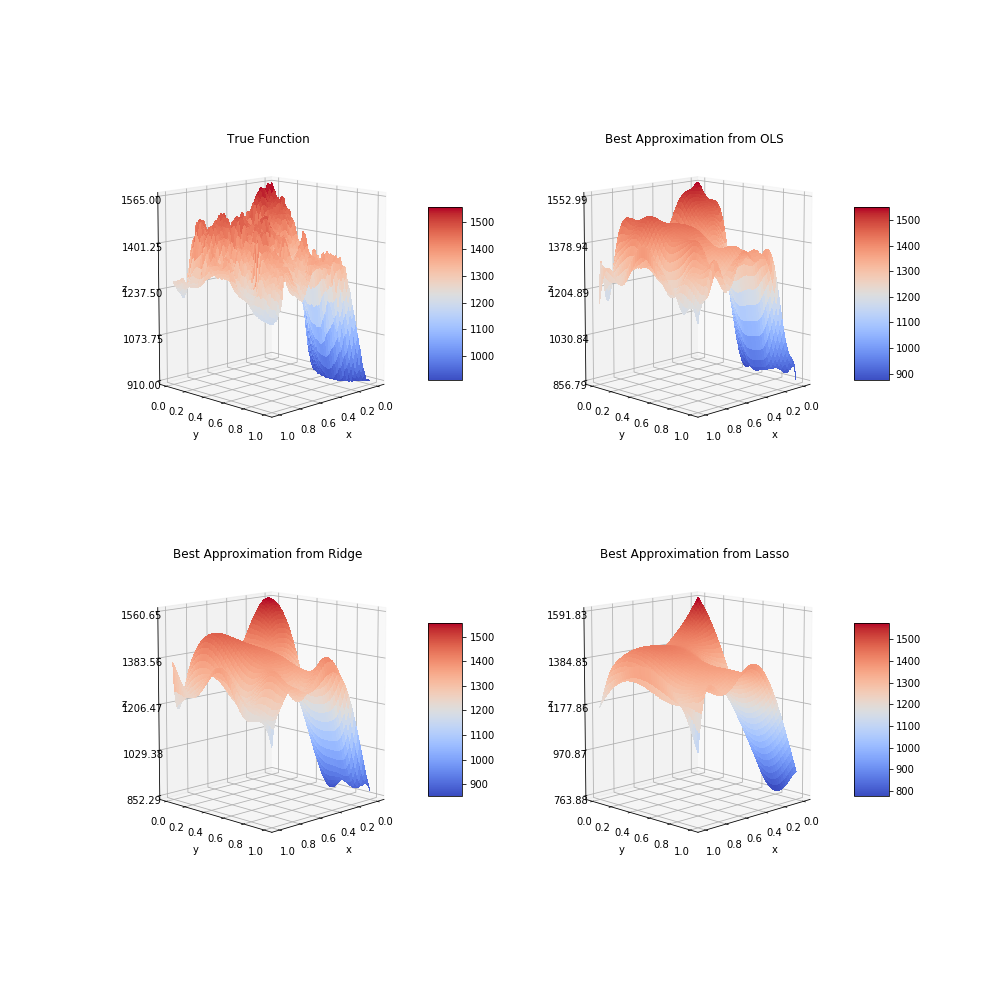
\includegraphics[scale=0.4]{Plots/PlotsRealData.png}
\caption{Prediction for terrain data}
\label{fig:realDataPlot}
\end{figure}

\clearpage

\begin{thebibliography}{3}
\bibitem{hasties}
Trevor Hastie, Robert Tibshirani and Jerome Friedman
\textit{The Elements of Statistical Learning}
Springer, Stanford, California, 2020

\bibitem{murphy}
Kevin P. Murphy
\textit{Machine Learning - A Probabilistic Perspective}
The MIT Press, Cambridge, Massachusetts, 2012

\bibitem{hjort}
Morten Hjort-Jensen: Linear Regression and Review of Statistical Analysis and Probability Theory 
\\\texttt{https://compphysics.github.io/MachineLearning/doc/pub/week35/html/week35.html}
2020

\bibitem{wessel}
Wessel N. van Wieringen: Lecture notes on ridge regression
\\\texttt{https://arxiv.org/pdf/1509.09169.pdf}
2020

\end{thebibliography}

\end{document}

